% !TEX TS-program = pdflatex
% !TEX encoding = UTF-8 Unicode

% This is a simple template for a LaTeX document using the "article" class.
% See "book", "report", "letter" for other types of document.

\documentclass[12pt]{book} % use larger type; default would be 10pt

\usepackage[utf8]{inputenc} % set input encoding (not needed with XeLaTeX)

%%% Examples of Article customizations
% These packages are optional, depending whether you want the features they provide.
% See the LaTeX Companion or other references for full information.

%%% PAGE DIMENSIONS
\usepackage[right=2cm,left=3cm,top=2cm,bottom=2cm,headsep=0cm,footskip=0.5cm]{geometry}
\usepackage{geometry} % to change the page dimensions
\geometry{a4paper} % or letterpaper (US) or a5paper or....
% \geometry{margin=2in} % for example, change the margins to 2 inches all round
% \geometry{landscape} % set up the page for landscape
%   read geometry.pdf for detailed page layout information

\usepackage{graphicx} % support the \includegraphics command and options

% \usepackage[parfill]{parskip} % Activate to begin paragraphs with an empty line rather than an indent

%%% PACKAGES
\usepackage{booktabs} % for much better looking tables
\usepackage{array} % for better arrays (eg matrices) in maths
%\usepackage{paralist} % very flexible & customisable lists (eg. enumerate/itemize, etc.)
\usepackage{verbatim} % adds environment for commenting out blocks of text & for better verbatim
\usepackage{subfig} % make it possible to include more than one captioned figure/table in a single float
% These packages are all incorporated in the memoir class to one degree or another...

%%% HEADERS & FOOTERS
\usepackage{fancyhdr} % This should be set AFTER setting up the page geometry
\pagestyle{fancy} % options: empty , plain , fancy
\renewcommand{\headrulewidth}{0pt} % customise the layout...
\lhead{}\chead{}\rhead{}
\lfoot{}\cfoot{\thepage}\rfoot{}

%%% SECTION TITLE APPEARANCE
\usepackage{sectsty}
\allsectionsfont{\sffamily\mdseries\upshape} % (See the fntguide.pdf for font help)
% (This matches ConTeXt defaults)

%%% ToC (table of contents) APPEARANCE
\usepackage[nottoc,notlof,notlot]{tocbibind} % Put the bibliography in the ToC
\usepackage[titles,subfigure]{tocloft} % Alter the style of the Table of Contents
\renewcommand{\cftsecfont}{\rmfamily\mdseries\upshape}
\renewcommand{\cftsecpagefont}{\rmfamily\mdseries\upshape} % No bold!

%%% Definiendo nuevos COLORES
\usepackage{xcolor} %Paquete de Color 
\definecolor{verde}{rgb}{0.25,0.5,0.35}
\definecolor{jpurple}{rgb}{0.5,0,0.35}

%%% Configurando el Layout para mostrar codigos Java
\usepackage{listings}
\lstset{
  language=Java,
  basicstyle=\ttfamily\small,
  keywordstyle=\color{jpurple}\bfseries,
  stringstyle=\color{red},
  commentstyle=\color{verde},
  morecomment=[s][\color{blue}]{/**}{*/},
  extendedchars=true,
  showspaces=false,
  showstringspaces=false,
  numbers=left,
  numberstyle=\tiny,
  breaklines=true,
  backgroundcolor=\color{cyan!10},
  breakautoindent=true,
  captionpos=b,
  xleftmargin=0pt,
  tabsize=3
}

%%% END Article customizations

\usepackage[spanish]{babel}
\usepackage{listings} 
\newcommand{\HRule}{\rule{\linewidth}{0.5mm}}
%%% The "real" document content comes below...


\title{Parsing XML with Haskell}
\author{Adriana Rodr\'iguez S\'anchez}

%\date{} % Activate to display a given date or no date (if empty),
         % otherwise the current date is printed 


\usepackage{eso-pic}
\newcommand\BackgroundEspol{
	\put(-218,338){
	\parbox[b][\paperheight]{\paperwidth}{%
           	\vfill
	           \centering
           	
\includegraphics[height=0.07\textheight,width=0.3\textwidth,keepaspectratio]{logoespol.jpg}%
	            \vfill
}}}

\newcommand\BackgroundFiec{
	\put(245,338){
	\parbox[b][\paperheight]{\paperwidth}{%
           	\vfill
	           \centering
           	
	            \vfill
}}}


\begin{document}


\begin{titlepage}
%\hspace*{0.2in}
\AddToShipoutPicture*{\BackgroundEspol}
\AddToShipoutPicture*{\BackgroundFiec}
%
\includegraphics[height=0.1\textheight]{logoespol}
%\hspace*{2.0in}
%
\includegraphics[width=0.3\textwidth]{logofiec}
%\includegraphics[width=0.1\textwidth]
\begin{center}
\textsc{\Large Escuela Superior Politécnica del Litoral}\\[1.0cm]
\textsc{\Large Facultad de Ingenieria en Electricidad y Computación}\\[1.5cm]

% Titulo
\HRule \\[0.4cm]
{ \LARGE \bfseries Parsing XML with Python \\[0.4cm] }
\HRule \\[1.5cm]


% Autores
\begin{minipage}{0.4\textwidth}
\begin{flushleft} \large
\emph{Autor:}\\
Adriana \textsc{Rodríguez}\\
\end{flushleft}
\end{minipage}
\begin{minipage}{0.4\textwidth}
\begin{flushright} \large
\emph{Profesor:} \\
Ing.~Javier \textsc{Tibau}
\end{flushright}
\end{minipage}
\vfill
% Bottom of the page
{\large \today}
\end{center}
\end{titlepage}





%\maketitle
\tableofcontents

\newpage
\mbox{}

\chapter{Introducci\'on}
XML es un lenguaje de marcado que permite almacenar datos, para ello esta conformado de una estructura abstracta para que as\'i se puedan trabajar con datos grandes.

En este caso, el prop\'osito de este documento es dar a conocer como en el lenguaje Haskell se puede trabajar para la administraci\'on de archivos XML y as\'i mostrar datos que sean espec\'ificos para el usuario. 

Para llevar un mejor control en los datos, decidimos trabajar por medio del \textit{parsing} que permite que los datos sean trabajados de una manera mas textual en la observaci\'on de todo el documento en si.

\begin{figure}[h!]
        \begin{center}
        
\includegraphics[scale=0.5]{pylogo.png}
        \end{center}
        \caption{Logo de Python.}
\end{figure}~\\[2cm]



\chapter{Alcance}
El alcance del proyecto es poder realizar un procesamiento de la informaci\'on que est\'a contenida en el archivo \textit{wurfl23.xml} y mostrar datos correspondientes a los dispositivos que cumplan con ciertas caracter\'isticas dichas por el usuario.

En este caso el parseo se lo llevar\'a a cabo por medio del lenguaje python. 


\begin{figure}[h!]
        \begin{center}
        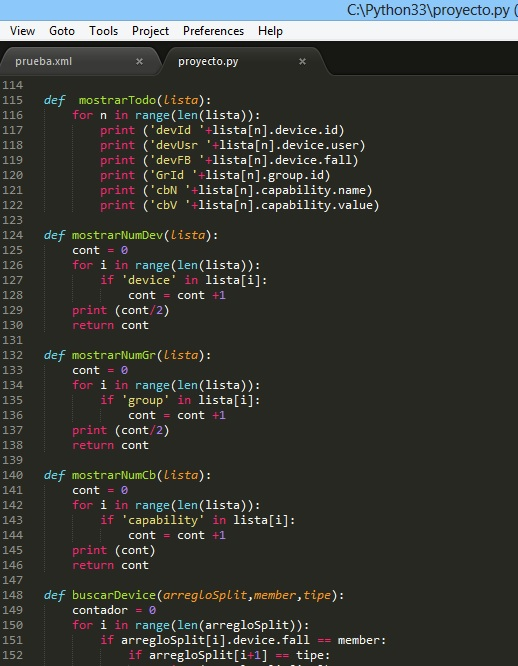
\includegraphics[scale=0.8]{pyex.jpg}
        \end{center}
        \caption{Codigo en Python.}
\end{figure}~\\[2cm]

\chapter{Descripci\'on}
El objetivo principal del proyecto es apreciar y entender las formas de programar en python.
Python es un lenguaje interpretado, todo trabaja con todo. Se puede decir que la manera de trabajar en python es mas sencilla en comparacion de Haskell ya que existe muchas herramientas que nos hacen posible el desarrollo del problema.~\\[0.5cm]

Los archivos XML trabajan por medio del marcado, llevan un control de los grupos de informaci\'on para asi mostrarlos como \textit{elementosl} que proporcionan una lista de estos elementos. El archivo antes mencionado, est\'a conformado por una serie elementos principales, estos son: Device, Group y los capability que son las listas principales que nos ayudar\'an a manipular los datos.~\\[0.5cm]

En el caso de los Device est\'an conformado por: 
\begin{itemize}
  \item id
  \item user agent
  \item fall back
\end{itemize}

A su vez, los Group est\'an conformado por: 
\begin{itemize}
  \item id
\end{itemize}

Y por \'ultimo los capability est\'an conformado por: 
\begin{itemize}
  \item name
  \item value
\end{itemize}


\chapter{Implementaci\'on}
El proyecto esta conformado por funciones y clases. Las clases estan conformadas por: Device, Group, Capability y General. Que contiene informacion de los atributos de cada tag en particular.~\\[0.5cm]
Las funciones son las encargadas de hacer la limpieza y la estructura de la informacion que deseamos manipular. Para este caso nos ayudamos mucho de varias funciones implementadas como son el replace, translate entre otros.~\\[0.5cm]


\chapter{Observaciones}
Cabe recalcar que para la realizacion de este proyecto se tuvo que reordenar los conocimientos, ya que en mi opinion Python trabaja de una manera muy diferente a otros lenguajes.~\\[0.5cm]
Uno de los problemas que tuve fue el ordenamiento creado al momento de crear las funciones, separandose con enter y no con tab.
\chapter{Conclusiones}
Python es \'util en varios aspectos como: 
\begin{itemize}
  \item Simplifica mucho la programación.
  \item Las librerías que más necesitas ya están dentro del código.
  \item Es un lenguaje ordenado.
\end{itemize}
\end{document}
